\begin{figure}[H]
    \centering


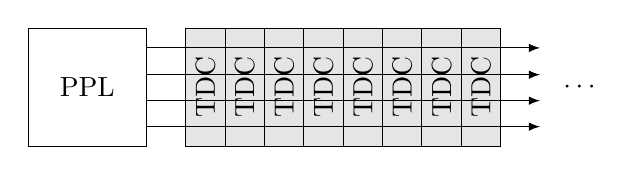
\begin{tikzpicture}

\draw  (-3.5,2.75) rectangle (-2,1.25) node[pos=.5]{PPL};

\draw [fill=gray!20] (-1.5,2.75) rectangle (-1,1.25) node[pos=.5, rotate=90]{TDC};
\draw [fill=gray!20] (-1,2.75) rectangle (-0.5,1.25) node[pos=.5, rotate=90]{TDC};
\draw [fill=gray!20] (-0.5,2.75) rectangle (0,1.25) node[pos=.5, rotate=90]{TDC};
\draw [fill=gray!20] (0,2.75) rectangle (0.5,1.25) node[pos=.5, rotate=90]{TDC};
\draw [fill=gray!20] (0.5,2.75) rectangle (1,1.25) node[pos=.5, rotate=90]{TDC};
\draw [fill=gray!20] (1,2.75) rectangle (1.5,1.25) node[pos=.5, rotate=90]{TDC};
\draw [fill=gray!20] (1.5,2.75) rectangle (2,1.25) node[pos=.5, rotate=90]{TDC};
\draw [fill=gray!20] (2,2.75) rectangle (2.5,1.25) node[pos=.5, rotate=90]{TDC};

\draw [>=latex, ->] (-2,2.5) -- (3,2.5);
\draw [>=latex, ->] (-2,2.16) -- (3,2.16);
\draw [>=latex, ->] (-2,1.83) -- (3,1.83);
\draw [>=latex, ->] (-2,1.5) -- (3,1.5);

\node at (3.5,2) {$\cdots$};
\end{tikzpicture}

    \caption{TDC line connected to PPL}
    \label{tkz:TDC_line_PPL}
\end{figure}